\section{Methodology}\label{sec:Methodology}

The methodology used in this research is summarized in the flowchart in \textbf{Figure \ref{fig:CH03_Methodology}}. 

\begin{figure}[h]
    \centering
    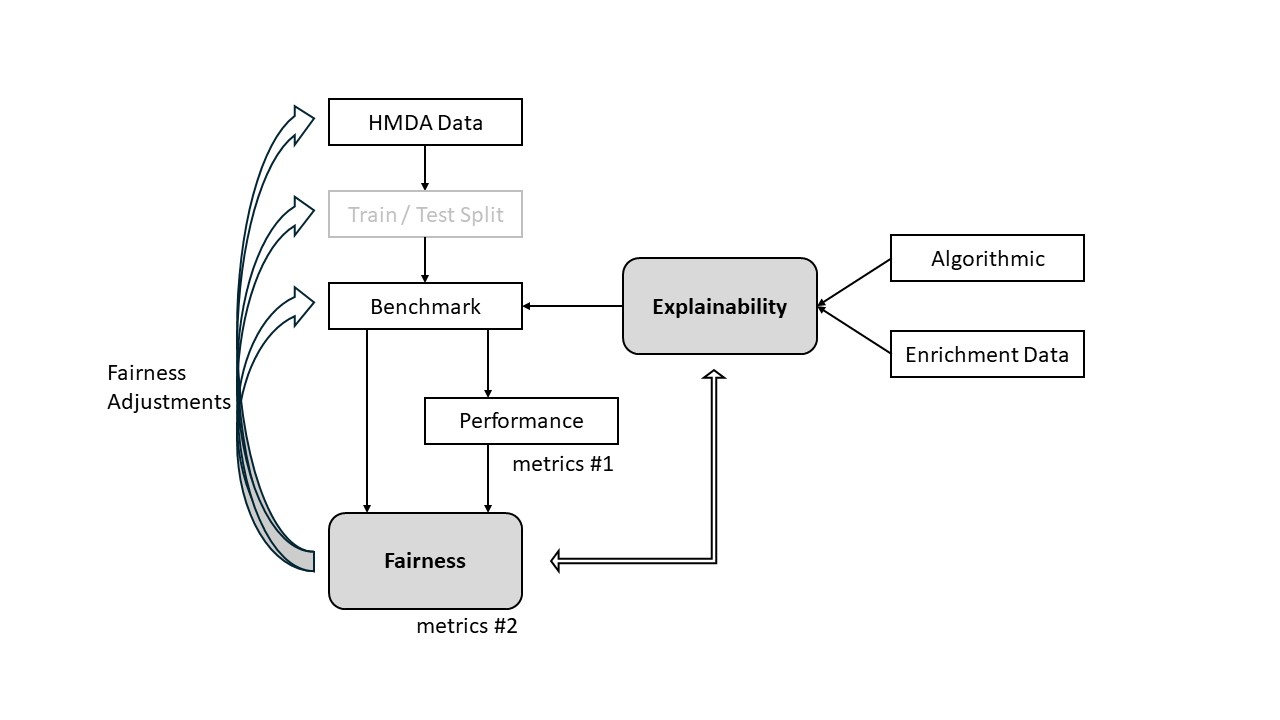
\includegraphics[width=0.85\textwidth]{CH03_Methodology.jpg}
    \caption{Methodology}
    \label{fig:CH03_Methodology}
\end{figure}

Data Preparation and Splitting have already been discussed in \textbf{Chapter \ref{subsec:Data_Preparation}}, details on the remaining steps will be provided in the following.

\subsection{Model Training and Prediction}\label{subsec:Model_Training_and_Prediction}

% Model choice
% Model setup details
% Model training process details
% Comment on debt_to_income_ratio imputation impacting accuracy but benefitting fairness (after reweighing)

\subsection{Explainability}\label{subsec:Explainability}

% Algorithm choice: Choice of model, reasoning, details of application
% Enrichment data: Explain use of geographical detail 

\subsection{Performance Assessment}\label{subsec:Performance_Assessment}

% Metrics: Choice of metrics, reasoning, details of application
% Cross-validation(?): Choice of method, reasoning, details of application

\subsection{Fairness Assessment}\label{subsec:Fairness_Assessment}

% Metrics: Choice of metrics, reasoning, details of application

\subsection{Iterations}\label{subsec:Iterations}

% Maybe more detail when decision has actually been made?
% Workflow idea: Training (unadjusted) -> Explainability -> Performance -> Fairness by using aequitas outcome (or checking AIF360) -> new technique by AIF 360 -> aim for similar performance but better fairness